\chapter{Introduction}
My fascination of retro computers sparked when I watched an online show about building an 8-bit computer on a breadboard. After countless hours of explanations, the viewer was rewarded with a blinking monster of wires and chips, functioning together to reach a goal. Ever since I watched this show \cite{beneater}, I wanted to design and build a computer like this. Over a couple of years I got further invested in the topic, fascinated by the initial impact of the first introduction of 8-bit computers in the 1970s and the sheer complexity of computer chips, I wanted to design my own computer architecture and simulation - just like if it was a real chip design, that is supposed to be physically manufactured on silicon. Unfortunately, physical construction, be it in silicon, or any other medium, was quickly ruled out due to overwhelming time efforts and costs. Manufacturing a chip in silicon not only requires physical manufacturing capabilities but also highly specialized software, that is proprietary and not intended for amateur usage. This paper is thus limited to all design steps before silicon or hardware design and manufacturing.

Following my inspiration, the architecture that is to be designed shall be kept very simple, in a way that is understandable by single person. This is achieved by limiting the bus width to 8-bits. Furthermore, the architecture shall follow the classic von Neumann Architecture and be Turing equivalent.  


\section{Chip Design} \label{sec:chip-design}
To move from idea to a finished product, chip designs follow a specific flow. Although different sources may describe this process differently, what is clear is, that this process is intended to be a highly sequential and linearized, which means, one step after the other. 

At first, all general requirements must be clearly established, which are then further broken down in smaller and smaller requirements. This step is referred to as "System specification and architectural design".

At some point these requirements then reach the point where, they specify functional details of the chip/architecture, such as compartmentalization and signaling. This is then referred to as "Functional design." With enough specificity these requirements can then be transferred into computer aided designs utilizing hardware description computer languages, a process called "Logic design". This logic design can then be transferred, either manually or by sophisticated computer programs, into logic gates and an on silicon layout, during the "physical design"  process. Before this is step is started, the logic design is tested against the defined requirements to ensure that it implements them correctly, which is called "Verification and Validation". Any mistakes in the logic design would translate into faulty silicon, making these mistakes extremely costly \cite{chipdesignflow1} \cite{chipdesignflow2}.

As previously stated, this project shall treat all steps up until and with "Verification and Validation". The collection of this process is sometimes also referred to \textit{front end design}.

\subsection{Requirements}
Requirements engineering describes the process of not only establishing high level requirements, e.g. the project goals, but also the translation into more specific and precise low level requirements. The formulation of useful requirements is essential to the success of a project. The value of a requirement lies in its ability to translate what the author wanted into what an engineer made of it. This means requirements must be unambiguous, correct and ideally precise and concise. \cite{cite.needed}

MORE

\subsection{Hardware Description Languages}
With the development of highly complex chip designs in the late 20th century further and further abstraction of the logic design process was required, ensuring that all stakeholders knew the exact specifications of the design at any point. \cite{1214355} Whilst the earliest chip designs were drawn by hand and late transferred onto silicon by photolithography, chip designs nowadays are first written in an abstract computer language; a Hardware Description Language. This hardware description can then be transferred into silicon either manually or automatically.  Apart from also allowing separation, modularity and reusability of components, this description later also allowed for simulation of the design. This simulation brought the key advantage of being able to be tested against requirements to check for errors.

\subsection{Automated Testing}
Nowadays, this automated testing process is handled by software frameworks designed for this purpose. These software frameworks instantiate and executes the simulation of the \textit{design under test} on top of \textit{testbench} code. The testbench models behavior of external components which is applied onto the design under test. The response of it is then compared to expected results and validated to ensure the design meets all requirements.

While requirements should cover all of an architectures' logic design implementation some pieces of code could be not covered by tests. To ensure that all code is tested, testing frameworks provide \textit{code coverage analysis tools}. The tools count activations of specific lines of code. This activation count can then be used to produce a visual report that shows all used lines of code, highlighting areas that aren't covered by code.

Automated test benches can be generally be split into two categories: exhaustive testing and directed testing. Exhaustive test benches test by supplying every possible test input to the design under test. 

\cite{verilogtestbenches} \cite{exhaustivetesting} \cite{directedtesting}


\subsection{Development Operations and Version Control Systems}
To track development over time \textit{version control systems} are used in basically every software project. Closely tied to most version control systems are \textit{development operations}. The goal of development operations is to connect the software development closer to its operations. In many projects these operations are e.g. the continuous deployment of code changes and the execution of the automated tests. Applied to this project, the development operations signify the execution of automatic testing of code changes as soon as changes are registered with the version control system. 

This combination allows for tracking and tracing the development process over time and provides quick feedback to engineers on problems arising in the code.

\section{Computer Architecture Design}
\subsection{Turing equivalence}
One of the most important concepts in computer science was established in 1936 by British mathematician Alan Turing. He described algorithm that is \texttt{computationally universal}. To be computationally universal an algorithm needs to be able to execute any other algorithm. \cite{britannicaturing} 

Given a number of theoretical problems in computer science an algorithm like this cannot exist. The most prominent example for this is the Halting Problem. It describes, that given computational universality, an algorithm needs to exist, that can determine another algorithms runtime. \cite{haltingproblem}

Computer science introduced the term \textit{Turing equivalent} to describe a machine that is exactly as powerful as the machine Turing described in his 1936 paper. If a computer architecture is Turing equivalent to a Turing machine, it can, given enough, theoretically infinite, memory, power and time, perform any algorithm that a modern computer can as well.

Lambda Calculus?

Generally speaking, to be Turing equivalent to a Turing machine, an architecture or machine must have the following capabilities \cite{beneaterturing}:
\begin{itemize}
  \item Have the ability to modify memory
  \item Have the ability to execute conditionally based on memory
  \item Have infinite time and memory
\end{itemize}


\subsection{The von Neumann Architecture}
In 1945 John von Neumann, an American mathematician, developed a concept for a computing device. What made this concept prevail into modern computing was its general purpose design. The executing program is intended to be exchangeable to fit the problem that is to be solved.

The truly pioneering approach of the von Neumann Architecture was to store the instructions in the same physical memory, thus accessed in the same way, as the data which simplified the programming process by allowing other programs (compilers, interpreters) to translate from more abstract languages. As instructions and data are stored in the same memory, they must also share the same physical bus. This however leads  to a phenomenon known as the \textit{von Neumann bottleneck}, where the bus and memory are the limiting factor in the speed of the computer. It arises because both the instruction fetch, and all data operations must share the same bus and can only occur one after the other, creating a point of congestion. 

The architecture is split up into four modules, that each serve a distinct purpose. The \textit{arithmetic logic unit} (ALU) handles all mathematical operations on data. All data is stored in the \textit{memory}. Interaction with users and/or other systems occur through the \textit{input/output unit}. All modules are orchestrated by the \textit{control unit} which controls the modules through the \textit{control bus}. The modules then exchange data through the \textit{data and address bus} \cite{vonneumann1} \cite{vonneumann2}.

\begin{figure}[H]
  \begin{center}
    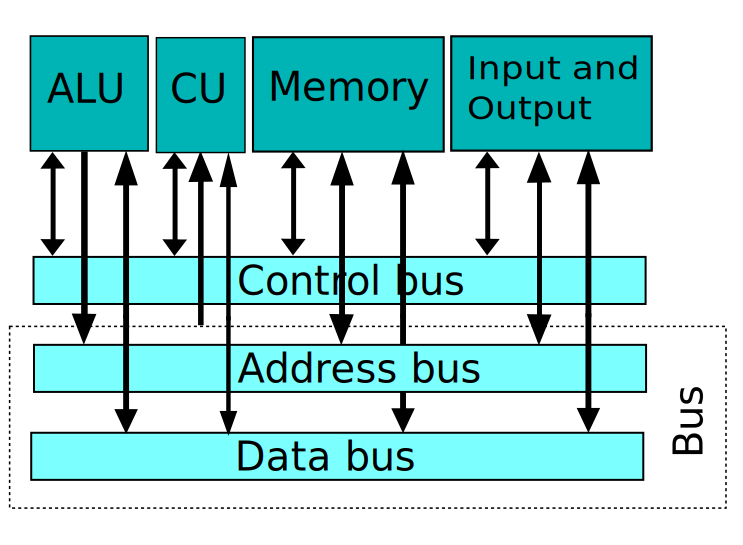
\includegraphics[width=0.5\textwidth]{figures/VNA}
  \end{center}
  \caption{The Von Neumann Architecture. Adapted from \cite{fig-vna}}\label{fig:vna}
\end{figure}

\subsection{Instruction Hierarchy}
The control unit controls the computer based on a \textit{program}. Each program serves a distinct purpose, e.g. calculating a series of numbers. It consists of multiple \textit{macro instructions}, which in return consist of multiple \textit{micro instructions}. Macro instructions perform, aligned with the von Neumann Architecture, an operation on a single \textit{data word}, such as overwriting it, or storing it somewhere else. A Micro instructions refers to the state of all control signals, e.g. if a component is reading or writing to the bus. Although it is possible to program a computer solely with micro instructions, it would be extremely inefficient, as the program code would be extremely repetitive. \cite{malvino1983a}

\section{Tools} \label{sec:tools}

The most popular flavor of such an \textit{HDL} is Verilog, as defined in \textit{IEEE Std 1800-2023} \cite{10458102} and its extensions. Given widespread professional use of Verilog, more specifically the Verilog superset SystemVerilog, seemed to be the best option for this project, a large amount of information and guides on the topic exist. The terms SystemVerilog and Verilog will be used interchangeably. 

As the IEEE Standard only defines the language's syntax, a Verilog tool suite is required. Although previous experience in the usage of Verilog exists, expertise on the intricacies of Verilog simulation is still limited. It was thus decided based on the integration with other tooling, as to which suite is to be used. 

The key feature of the chosen suite, which is called \textit{Verilator}, is the compilation of the Verilog code to a binary and the generation of an interface to C++. Having an interface to C++ enables much more complex behaviors to be modeled simpler, such as reading test data from a file. Additionally, apart from being able to rely on previous experience in C++, it also allows me to make use of a vast ecosystem of testing, code coverage and development operations frameworks. Furthermore, the suite is available under the LGPL license, allowing me to use it free of charge. I chose the GoogleTest framework for automated testing procedures. Most testing frameworks in essence do the same thing, although there are small nuances that differ from one to the other. 

Verilator also provides interfaces to coverage analysis tools by generating \textit{dumpfiles}. Dumpfiles contain the data of all signal values in the simulation across time and can be read by "digital oscilloscopes" like \texttt{GTKWave}. These can then be used to debug and understand the simulation, in case errors exist \cite{verilatoroverview}.

Git and GitLab are used as the version control system and development operations platform.

\subsection{Verilog Crash Course}
This section is not intended to be an exhaustive guide to Verilog, but only highlights the most important features and concepts, relevant for this project.

What differentiates simulated Verilog from other computer languages is its non-linear execution and lacks the concept of a main function. Verilog files are not necessarily executed from top to bottom, but execution is based on propagation of signals throughout the interconnected modules. 

A module is declared with the \texttt{module} keyword. To complete a declaration the module must be named and ports specified. Ports are the connections going in and out of a module. They can either be an \texttt{input}, an \texttt{output} or bidirectional, denoted by \texttt{inout}. Ports are then specified like any other variable, by specifying the datatype, length and name. For this paper usage of data types shall be limited to, \texttt{wire}, \texttt{reg}, \texttt{logic} and for readability reasons \texttt{enum}. After the declaration of the ports the body of the module is defined, which contains the module logic.

\begin{lstlisting}[language=Verilog, caption=Module definition]
module <module_name> (
  input wire <input_name>,
  output reg <output_name>
);
<module_body>
endmodule
\end{lstlisting}


Most digital circuits are based around a clock signal and thus have to execute operations at every clock cycle. Verilog provides a way to model this with \texttt{always} blocks. Once the condition in the bracket is met, the code block is executed. Apart from simple boolean conditions, the block can also be executed at the rising and falling edge of a signal by using the \texttt{posedge} and \texttt{negedge} keywords.

\begin{lstlisting}[language=Verilog, caption=Always block definition]
always @(<condition>) begin
  <always_body>
end

\end{lstlisting}

For logic the Verilog standard specifies comparable to other computer or programming languages if-blocks, loops, case statements and various logic and arithmetic operators. Unlike other languages, there are multiple types of assignments in Verilog. The easiest to understand is the continuous assignment with the \texttt{assign} keyword. This continuously assigns the value of the right-hand side to the left-hand side comparable to physical wires being connected together through logic gates. If the input changes, the output will change with it nearly instantaneously. The blocking assignment, denoted by the \texttt{=} operator, is used to assign values to variables instantaneously, like in other programming languages. The non-blocking assignment, denoted by the \texttt{<=} operator, only actually assigns the value to the left-hand side once the timing step, so every calculation in the current time step, is finished. 

The SystemVerilog standard also specifies a number of additional functions that are not synthesizable, so cannot be translated into hardware, but are useful for simulation, such as \texttt{\$display} and \texttt{\$finish}. As they are not synthesizable, they shall not be used, for this project. These features can be handled by the \texttt{C++} testbenches.

\cite{verilogcourse}

\subsection{Development Environment}
To reproduce the development environment for this project, the following packages need to be available in \texttt{PATH}. I suggest to use Debian 12. 

\begin{itemize}
  \item verilator@5.24
  \item a C++ tool chain (e.g. GCC)
  \item CMake
  \item a CMake generator (e.g. ninja)
\end{itemize}  

\section{Idea and Goal} \label{sec:goal}  
The following list can be understood as the "high(est) level requirements" to this project:
\begin{itemize}
  \item Have a functioning computer architecture that:
 \begin{enumerate}
    \item Has an 8-bit bus width
    \item Is Turing equivalent
    \item Is based on the von Neumann Architecture
    \item Implements features wanted by me
    \item Is kept as simple as possible
    \item Is, with supporting work, explainable graphically
  \end{enumerate}
  \item Have a simulation of this computer architecture that: 
  \begin{enumerate}
    \item Is fully tested, ensuring all requirements are met
    \item Is kept as simple as possible
    \item Can be interacted with by a user
    \item Is programmable by a higher level language (assembly)
    \item Is, with supporting work, explainable graphically.
  \end{enumerate}
\end{itemize}

Additionally, the process shall occur in a traceable process, that is aligned to the process described in \ref{sec:chip-design}.

Implementation and execution of these goals shall be analyzed in chapter \ref{chap:conclusion}.

Features that are wanted by me are intended to increase the feature set of the architecture to make it more useable and may or may not be based on my subjectivity.